\section{Тема 5. Сетевое планирование проекта}

Сетевое планирование и управление (СПУ), система планирования и управления разработкой крупных народно-хозяйственных комплексов, научными исследованиями, конструкторской и технологической подготовкой производства новых видов изделий, строительством и реконструкцией, капитальным ремонтом основных фондов путём применения сетевых графиков. Система СПУ позволяет устанавливать взаимосвязь планируемых работ и получаемых результатов, более точно рассчитывать план, а также своевременно осуществлять его корректировку. СПУ --- основа использования ЭВМ в управлении и создании АСУ.

Сущность СПУ состоит в составлении логико-математической модели управляемого объекта в виде сетевого графика (рисунок \ref{fig:seti}) или модели, находящейся в памяти ЭВМ, в которой отражаются взаимосвязь и длительность определённого комплекса работ. Сетевой график после его оптимизации средствами прикладной математики и вычислительной техники используется для оперативного управления работами.
\begin{figure}[!h]
	\centering
	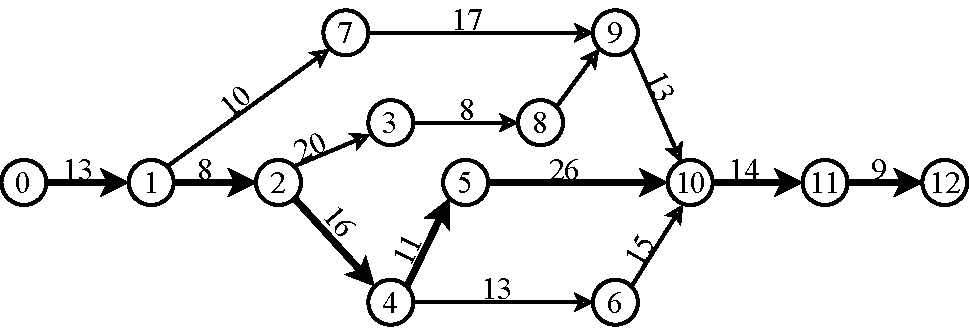
\includegraphics[width=0.7\linewidth]{seti}
	\caption{Сетевой график}
	\label{fig:seti}
\end{figure}

На график нанесены работы и события. Каждое событие характеризует завершение или начало работы, а работа означает действие, которое нужно совершить, чтобы перейти от предшествующего события к последующему. События на графике обозначаются кружками, а работы --- стрелками, показывающими связь между событиями (возможен и другой вариант: работы изображаются кружками, а связи между ними стрелками). Работа должна быть конкретной, четко описанной и иметь ответственного исполнителя; продолжительность её измеряется количеством дней, недель, декад и др., наносимых над стрелкой. Временные оценки даются ответственными исполнителями соответствующих работ. Все работы в графике ведут к конечному событию --- цели планирования.

При планировании длительности работ пользуются действующими нормативами и опытными данными, но во многих случаях (в частности, когда рассматриваются программы по освоению новых видов продукции или проблемные научные исследования) время работы не может быть выражено одной достоверной оценкой; ответственный исполнитель обычно даёт 3 оценки. Оптимистическая оценка времени (минимальная продолжительность работы $t_{min}$) --- минимальный срок, в течение которого будет выполнена работа в наиболее благоприятных условиях, если ничто не помешает её выполнению. Пессимистическая оценка времени (максимальная продолжительность работы $t_{max}$) характеризуется продолжительностью времени, необходимого для выполнения работы при наиболее неблагоприятных условиях, если в процессе её выполнения возникнут трудности. Наиболее вероятная продолжительность времени ($t_{\text{нв}}$) показывает время выполнения работы в нормальных условиях.

Ожидаемая продолжительность работы определяется на основании 3 или 2 оценок по одной из следующих формул:
\[t_{\text{ож}} =\dfrac{t_{min} + 4 \cdot t_{\text{нв}} + t_{max}}{6}\  \text{или} \  t_{\text{ож}} = \dfrac{3 \cdot t_{min}  +2 \cdot t_{max} }{5} \]
 

Важный элемент разработки сетевого графика --- определение продолжительности путей. На рисунке \ref{fig:seti} пути представлены линиями, образуемыми стрелками взаимосвязанных работ, концы которых указывают на начальные и конечные события. Различают полные и критические пути: полным называется путь, начало которого совпадает с исходным событием сети, а конец --- с её завершающим событием; критическим --- путь, имеющий наибольшую продолжительность и характеризующий время выполнения всего комплекса работ, проекта в целом, т. е. время достижения конечной цели (на рисунке обозначен жирными стрелками).

Критический путь расценивается как самый важный в системе СПУ, т. к. представляет собой основу для выбора оптимального плана и организации контроля за ходом работ. Отношение продолжительности любого пути к продолжительности критического пути характеризует степень его напряжённости. Если критический путь является наиболее продолжительным по времени от начального до конечного события, то все др. события и работы должны лежать на путях более коротких.

Совершенные формы СПУ содержат информацию относительно движения материальных затрат и наращивания издержек по объекту. СПУ проводится примерно в следующей очерёдности: расчленение комплекса работ на отдельные последовательные этапы, каждый из которых закрепляется за ответственным исполнителем; выявление и описание всех событий и работ, необходимых для достижения неконечной цели; построение сетевого графика; определение времени выполнения каждой работы в сети на основе системы оценок; расчёт критического пути и резервов времени; анализ сети и оптимизация графика, разработка мероприятий по сокращению времени критического пути; управление ходом работ с помощью сетевого графика.

Каждый исполнитель определяет состав и последовательность закрепленного за ним этапа работ. Затем ответственное за проект лицо составляет первичные сетевые графики, которые после их корректировки «сшиваются» в сводный сетевой график. Этот график завершается событием, соответствующим заданной конечной цели. При этом особое внимание уделяется устранению неувязок на стыках между первичными сетевыми графиками, т. е. этапами комплекса работ.

По мере движения ко всё более высокому уровню выполнения работ планы-графики укрупняются. Если они предназначены для руководителей предприятий, то в них включаются только сроки свершения граничных событий, являющихся выходными для одних предприятий и входными для других, с указанием времени начала и окончания работ критической зоны. Планы-графики руководителей промежуточных ступеней дополняются сведениями о сроках свершения граничных событий между отдельными ответственными исполнителями.

В процессе выполнения планов-графиков осуществляются непрерывный контроль, корректировка и регулирование сетевой модели. Для устранения расхождений между запланированным и фактическим ходом работ проводятся организационно-технические мероприятия.

Т. о., СПУ создаёт в конечном счёте условия для выполнения всего комплекса работ в их логической последовательности. С помощью сетевых графиков осуществляется системный подход к вопросам организации управления заданными процессами, поскольку коллективы различных подразделений участвуют в них как звенья единой сложной организационной системы, объединённые общностью задачи.